\section{Emboss}

\begin{frame}
    \frametitle{Emboss\footnote{\url{http://faculty.ycp.edu/~dhovemey/spring2011/cs365/labs/lab6.html}}}

    \begin{itemize}
        \item Jeder Pixel $ p^{rgba}_{ij} $ wird mit oben-links liegendem Pixel $ p^{rgba}_{i-1j-1} $ verglichen \pause
        \item Die größte, absolute Differenz wird als Referenzwert genommen
        \item $ d_{ij} = max(|p^{r}_{ij} - p^{r}_{i-1j-1}|, |p^{g}_{ij} - p^{g}_{i-1j-1}|, |p^{b}_{ij} - p^{b}_{i-1j-1}|) $ \pause
        \item Die Werte der Channels für den neuen Pixel entsprechenden dem Referenzwert addiert mit 128 und beschränkt auf 0-255, der Alpha-Channel vom Ausgangspixel übernommen \pause
        \item $ p' = min(0, max(255, d_{ij} + 128)) $
    \end{itemize}
\end{frame}

\begin{frame}
    \frametitle{Emboss - Ergebnisse 1}

    \begin{itemize}
        \item dice.png
        \item 800 x 600
        \item 295 KB
    \end{itemize}

    \hfill
    \hrule
    \hfill

    \begin{figure}[H]
        \centering
    
        \includegraphics[width=0.30\textwidth]{images/dice.png}
        \includegraphics[width=0.30\textwidth]{images/results/emboss-my.dice.png}

        
        \begin{center}
            \caption{Emboss results of self-implemented Algorithm (right)}
        \end{center}

        \label{fig:emboss1}
    \end{figure}
\end{frame}

\begin{frame}
    \frametitle{Emboss - Performance 1}

    \begin{center}
    \begin{figure}[H]
        \centering

        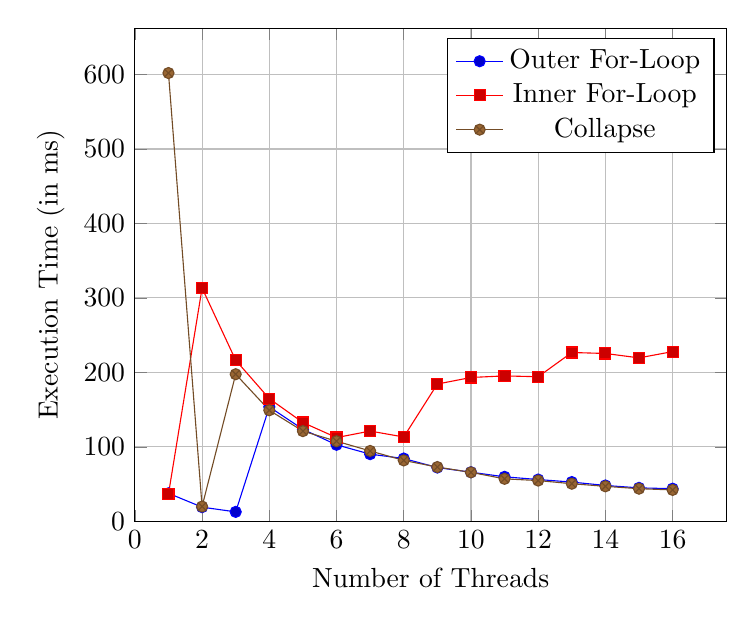
\begin{tikzpicture}
            \begin{axis}[
                title={},
                width=0.75\textwidth,
                xlabel={Number of Threads},
                ylabel={Execution Time (in ms)},
                xmin=0,
                ymin=0,
                grid=major
            ]
                \addplot coordinates {
                    (1,37.6192)(2,19.0143)(3,12.6701)(4,153.6)(5,123.528)(6,102.743)(7,90.193)(8,84.3286)(9,72.2025)(10,65.9573)(11,59.7616)(12,56.1131)(13,52.7063)(14,48.1298)(15,44.9207)(16,43.8277)
                };
                \addlegendentry{Outer For-Loop}

                \addplot coordinates {
                    (1,36.5978)(2,313.246)(3,216.304)(4,164.724)(5,132.658)(6,112.436)(7,121.197)(8,113.254)(9,184.333)(10,193.15)(11,195.278)(12,194.14)(13,226.703)(14,225.382)(15,219.47)(16,227.906)
                };
                \addlegendentry{Inner For-Loop}       

                \addplot coordinates {
                    (1,601.954)(2,19.8608)(3,197.528)(4,149.097)(5,121.117)(6,107.558)(7,94.5198)(8,81.7579)(9,72.864)(10,65.7456)(11,57.0341)(12,54.7264)(13,50.4797)(14,46.9844)(15,43.8079)(16,42.1596)
                };
                \addlegendentry{Collapse}
            \end{axis}
        \end{tikzpicture}
        \caption{Emboss Performance Tests dice.png}
    \end{figure}
\end{center}

\end{frame}

\begin{frame}
    \frametitle{Emboss - Ergebnisse 2}

    \begin{itemize}
        \item dice\_large.png
        \item 1754 x 1554
        \item 1.5 MB
    \end{itemize}

    \hfill
    \hrule
    \hfill

    \begin{figure}[H]
        \centering
    
        \includegraphics[width=0.30\textwidth]{images/dice_large.png}
        \includegraphics[width=0.30\textwidth]{images/results/emboss-my.dice_large.png}

        
        \begin{center}
            \caption{Emboss results of self-implemented Algorithm (right)}      
        \end{center}

        \label{fig:emboss2}
    \end{figure}
\end{frame}

\begin{frame}
    \frametitle{Emboss - Performance 2}

    \begin{center}
    \begin{figure}[H]
        \centering

        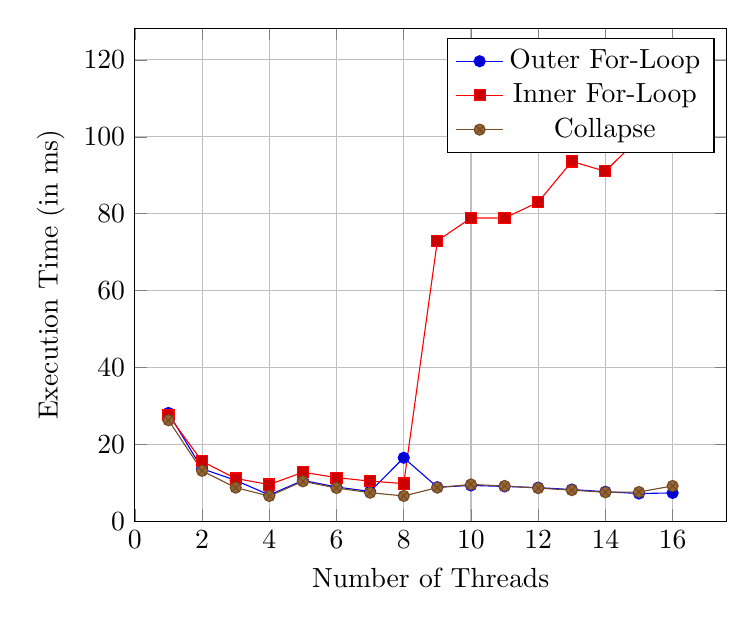
\begin{tikzpicture}
            \begin{axis}[
                title={},
                width=0.75\textwidth,
                xlabel={Number of Threads},
                ylabel={Execution Time (in ms)},
                xmin=0,
                ymin=0,
                grid=major
            ]
                \addplot coordinates {
                    (1,28.1787)(2,13.6684)(3,10.6587)(4,6.841)(5,10.6448)(6,8.9229)(7,7.7613)(8,16.5284)(9,8.8759)(10,9.3305)(11,9.0727)(12,8.75325)(13,8.265)(14,7.6939)(15,7.22555)(16,7.37725)
                };
                \addlegendentry{Outer For-Loop}

                \addplot coordinates {
                    (1,27.5487)(2,15.6059)(3,11.1323)(4,9.5563)(5,12.7669)(6,11.3685)(7,10.444)(8,9.8202)(9,72.9501)(10,78.8844)(11,78.8677)(12,82.9903)(13,93.5949)(14,91.0306)(15,99.7156)(16,116.585)
                };
                \addlegendentry{Inner For-Loop}       

                \addplot coordinates {
                    (1,26.2787)(2,13.1285)(3,8.74935)(4,6.5788)(5,10.3955)(6,8.6642)(7,7.436)(8,6.6008)(9,8.76145)(10,9.5894)(11,9.1864)(12,8.6334)(13,8.10475)(14,7.5467)(15,7.62205)(16,9.2002)
                };
                \addlegendentry{Collapse}
            \end{axis}
        \end{tikzpicture}
        \caption{Emboss Performance Tests dice.png}
    \end{figure}
\end{center}

\end{frame}

\begin{frame}
    \frametitle{Emboss - Ergebnisse 3}

    \begin{itemize}
        \item pnglogo-blk.png
        \item 1024 x 768
        \item 516 KB
    \end{itemize}

    \hfill
    \hrule
    \hfill

    \begin{figure}[H]
        \centering
    
        \includegraphics[width=0.30\textwidth]{images/pnglogo-blk.png}
        \includegraphics[width=0.30\textwidth]{images/results/emboss-my.pnglogo-blk.png}

        
        \begin{center}
            \caption{Emboss results of self-implemented Algorithm (right)}
        \end{center}

        \label{fig:emboss3}
    \end{figure}
\end{frame}

\begin{frame}
    \frametitle{Emboss - Performance 3}

    \begin{center}
    \begin{figure}[H]
        \centering

        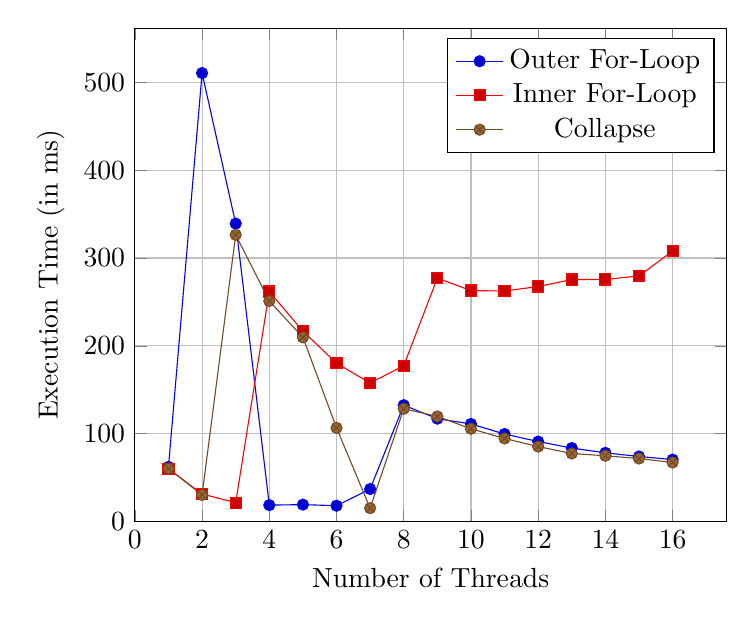
\begin{tikzpicture}
            \begin{axis}[
                title={},
                width=0.75\textwidth,
                xlabel={Number of Threads},
                ylabel={Execution Time (in ms)},
                xmin=0,
                ymin=0,
                grid=major
            ]
                \addplot coordinates {
                    (1,61.9455)(2,510.799)(3,339.263)(4,18.4507)(5,19.0326)(6,17.7779)(7,36.7884)(8,132.337)(9,116.961)(10,110.943)(11,99.4424)(12,90.9082)(13,83.4689)(14,78.0252)(15,73.8739)(16,70.3217)
                };
                \addlegendentry{Outer For-Loop}

                \addplot coordinates {
                    (1,60.0459)(2,31.0737)(3,21.2645)(4,261.838)(5,216.725)(6,180.175)(7,157.577)(8,177.301)(9,277.111)(10,262.917)(11,262.411)(12,267.611)(13,275.478)(14,275.589)(15,279.614)(16,308.027)
                };
                \addlegendentry{Inner For-Loop}       

                \addplot coordinates {
                    (1,60.0662)(2,30.0693)(3,326.473)(4,251.054)(5,209.641)(6,106.486)(7,14.9989)(8,128.224)(9,119.544)(10,105.455)(11,94.4388)(12,85.1538)(13,77.2811)(14,74.681)(15,71.526)(16,66.9778)
                };
                \addlegendentry{Collapse}
            \end{axis}
        \end{tikzpicture}
        \caption{Emboss Performance Tests pnglogo-blk.png}
    \end{figure}
\end{center}

\end{frame}